% Created 2019-01-31 Thu 22:22
% Intended LaTeX compiler: pdflatex
\ifdefined\kanjiskip
                                                   \documentclass[autodetect-engine,dvipdfmx,12pt,a4paper,ja=standard]{bxjsarticle}
                                                 \else
                                                   \ifdefined\pdfoutput
                                                     \ifnum\pdfoutput=0
                                                       \documentclass[autodetect-engine,dvipdfmx,12pt,a4paper,ja=standard]{bxjsarticle}
                                                     \else
                                                       \documentclass[autodetect-engine,12pt,a4paper,ja=standard]{bxjsarticle}
                                                     \fi
                                                   \else
                                                     \documentclass[autodetect-engine,12pt,a4paper,ja=standard]{bxjsarticle}
                                                   \fi
                                                 \fi
                                                 \usepackage{amsmath}
                                                 \usepackage{newtxtext,newtxmath}
                                                 \usepackage{graphicx}
                                                 \usepackage{hyperref}
                                                 \ifdefined\kanjiskip
                                                 \usepackage{pxjahyper}
                                                 \hypersetup{colorlinks=true}
                                                 \else
                                                 \ifdefined\XeTeXversion
                                                 \hypersetup{colorlinks=true}
                                                 \else
                                                 \ifdefined\directlua
                                                 \hypersetup{pdfencoding=auto,colorlinks=true}
                                                 \else
                                                 \hypersetup{unicode,colorlinks=true}
                                                 \fi
                                                 \fi
                                                 \fi
\author{細田弘吉}
\date{\today}
\title{}
\hypersetup{
 pdfauthor={細田弘吉},
 pdftitle={},
 pdfkeywords={},
 pdfsubject={},
 pdfcreator={Emacs 26.1 (Org mode 9.1.13)},
 pdflang={English}}
\begin{document}

\tableofcontents


\section{Home}
\label{sec:org85fdb33}

\section{Posts}
\label{sec:org9af93a1}
\subsection{Emacsの長い行を折り返して見やすくするが実際の行は変えない.adaptive-wrap --- Correct indentation for wrapped lines\hfill{}\textsc{emacs:org\_mode:adaptive:wrap:indentation}}
\label{sec:org2305e8f}
Emacsで長い行を書いていると,デフォルトの状態ではどんどん横に伸びていく.後で読み返そうと思うと横にスクロールしないといけなくて,非常に不便である.M-qでauro-fillをやればよいと言われそうだが,そうすると改行されてしまい,これまた不便である.そこで,なんとかならないかと探してみると,ちゃんとそういうモノがあったので,まとめておく.

\setcounter{tocdepth}{2}
\tableofcontents

\subsubsection{adaptive-wrap}
\label{sec:org791cf7e}
\begin{itemize}
\item 参照1:\href{https://elpa.gnu.org/packages/adaptive-wrap.html}{adaptive-wrap} \footnote{\url{https://elpa.gnu.org/packages/adaptive-wrap.html}}  ご本家
\item 参照2:\href{https://emacs.stackexchange.com/questions/14589/correct-indentation-for-wrapped-lines}{Correct indentation for wrapped lines} \footnote{\url{https://emacs.stackexchange.com/questions/14589/correct-indentation-for-wrapped-lines}}
\item 参照3:\href{http://alainmathematics.blogspot.com/2013/07/emacs.html}{Emacsの折り返しの挙動} \footnote{\url{http://alainmathematics.blogspot.com/2013/07/emacs.html}}
\item 参照4:\href{https://www.reddit.com/r/emacs/comments/1kw7ip/emacs_settings_loading_issue/}{.emacs settings loading issue} \footnote{\url{https://www.reddit.com/r/emacs/comments/1kw7ip/emacs_settings_loading_issue/}}  
\end{itemize}

長い行をワープロのようにword-wrapしてくれるパッケージである.Emacsのバッファ上では折り返されているように見えるが,実際は長い横1行のままである.

\begin{enumerate}
\item インストールと設定
\label{sec:orga649958}
例によって,use-packagを用いて以下のように,init.orgに書けばよい.
\begin{verbatim}
#+begin_src emacs-lisp
(use-package adaptive-wrap
  :ensure t
  :config
  (setq-default adaptive-wrap-extra-indent 1)
  (add-hook 'visual-line-mode-hook #'adaptive-wrap-prefix-mode)
  (global-visual-line-mode +1)
  (add-hook 'org-mode-hook 'visual-line-mode)  ;; For
  )
#+end_src
\end{verbatim}

なお,最後の行を入れておかないと,org-mode fileに

\begin{verbatim}
#+setupfile: /Sources/org-mode-folder/org-macros-master/org-macros.setup
\end{verbatim}

を追加してマクロのパッケージを使用する場合(\href{../html_export}{Emacsのorg-modeで論文を書く(その5:htmlへのexportの際のフォントの色の変更,ハイライトなど)(12月19日追記)}を参照のこと)に,adaptive-wrapが効かなくなる.

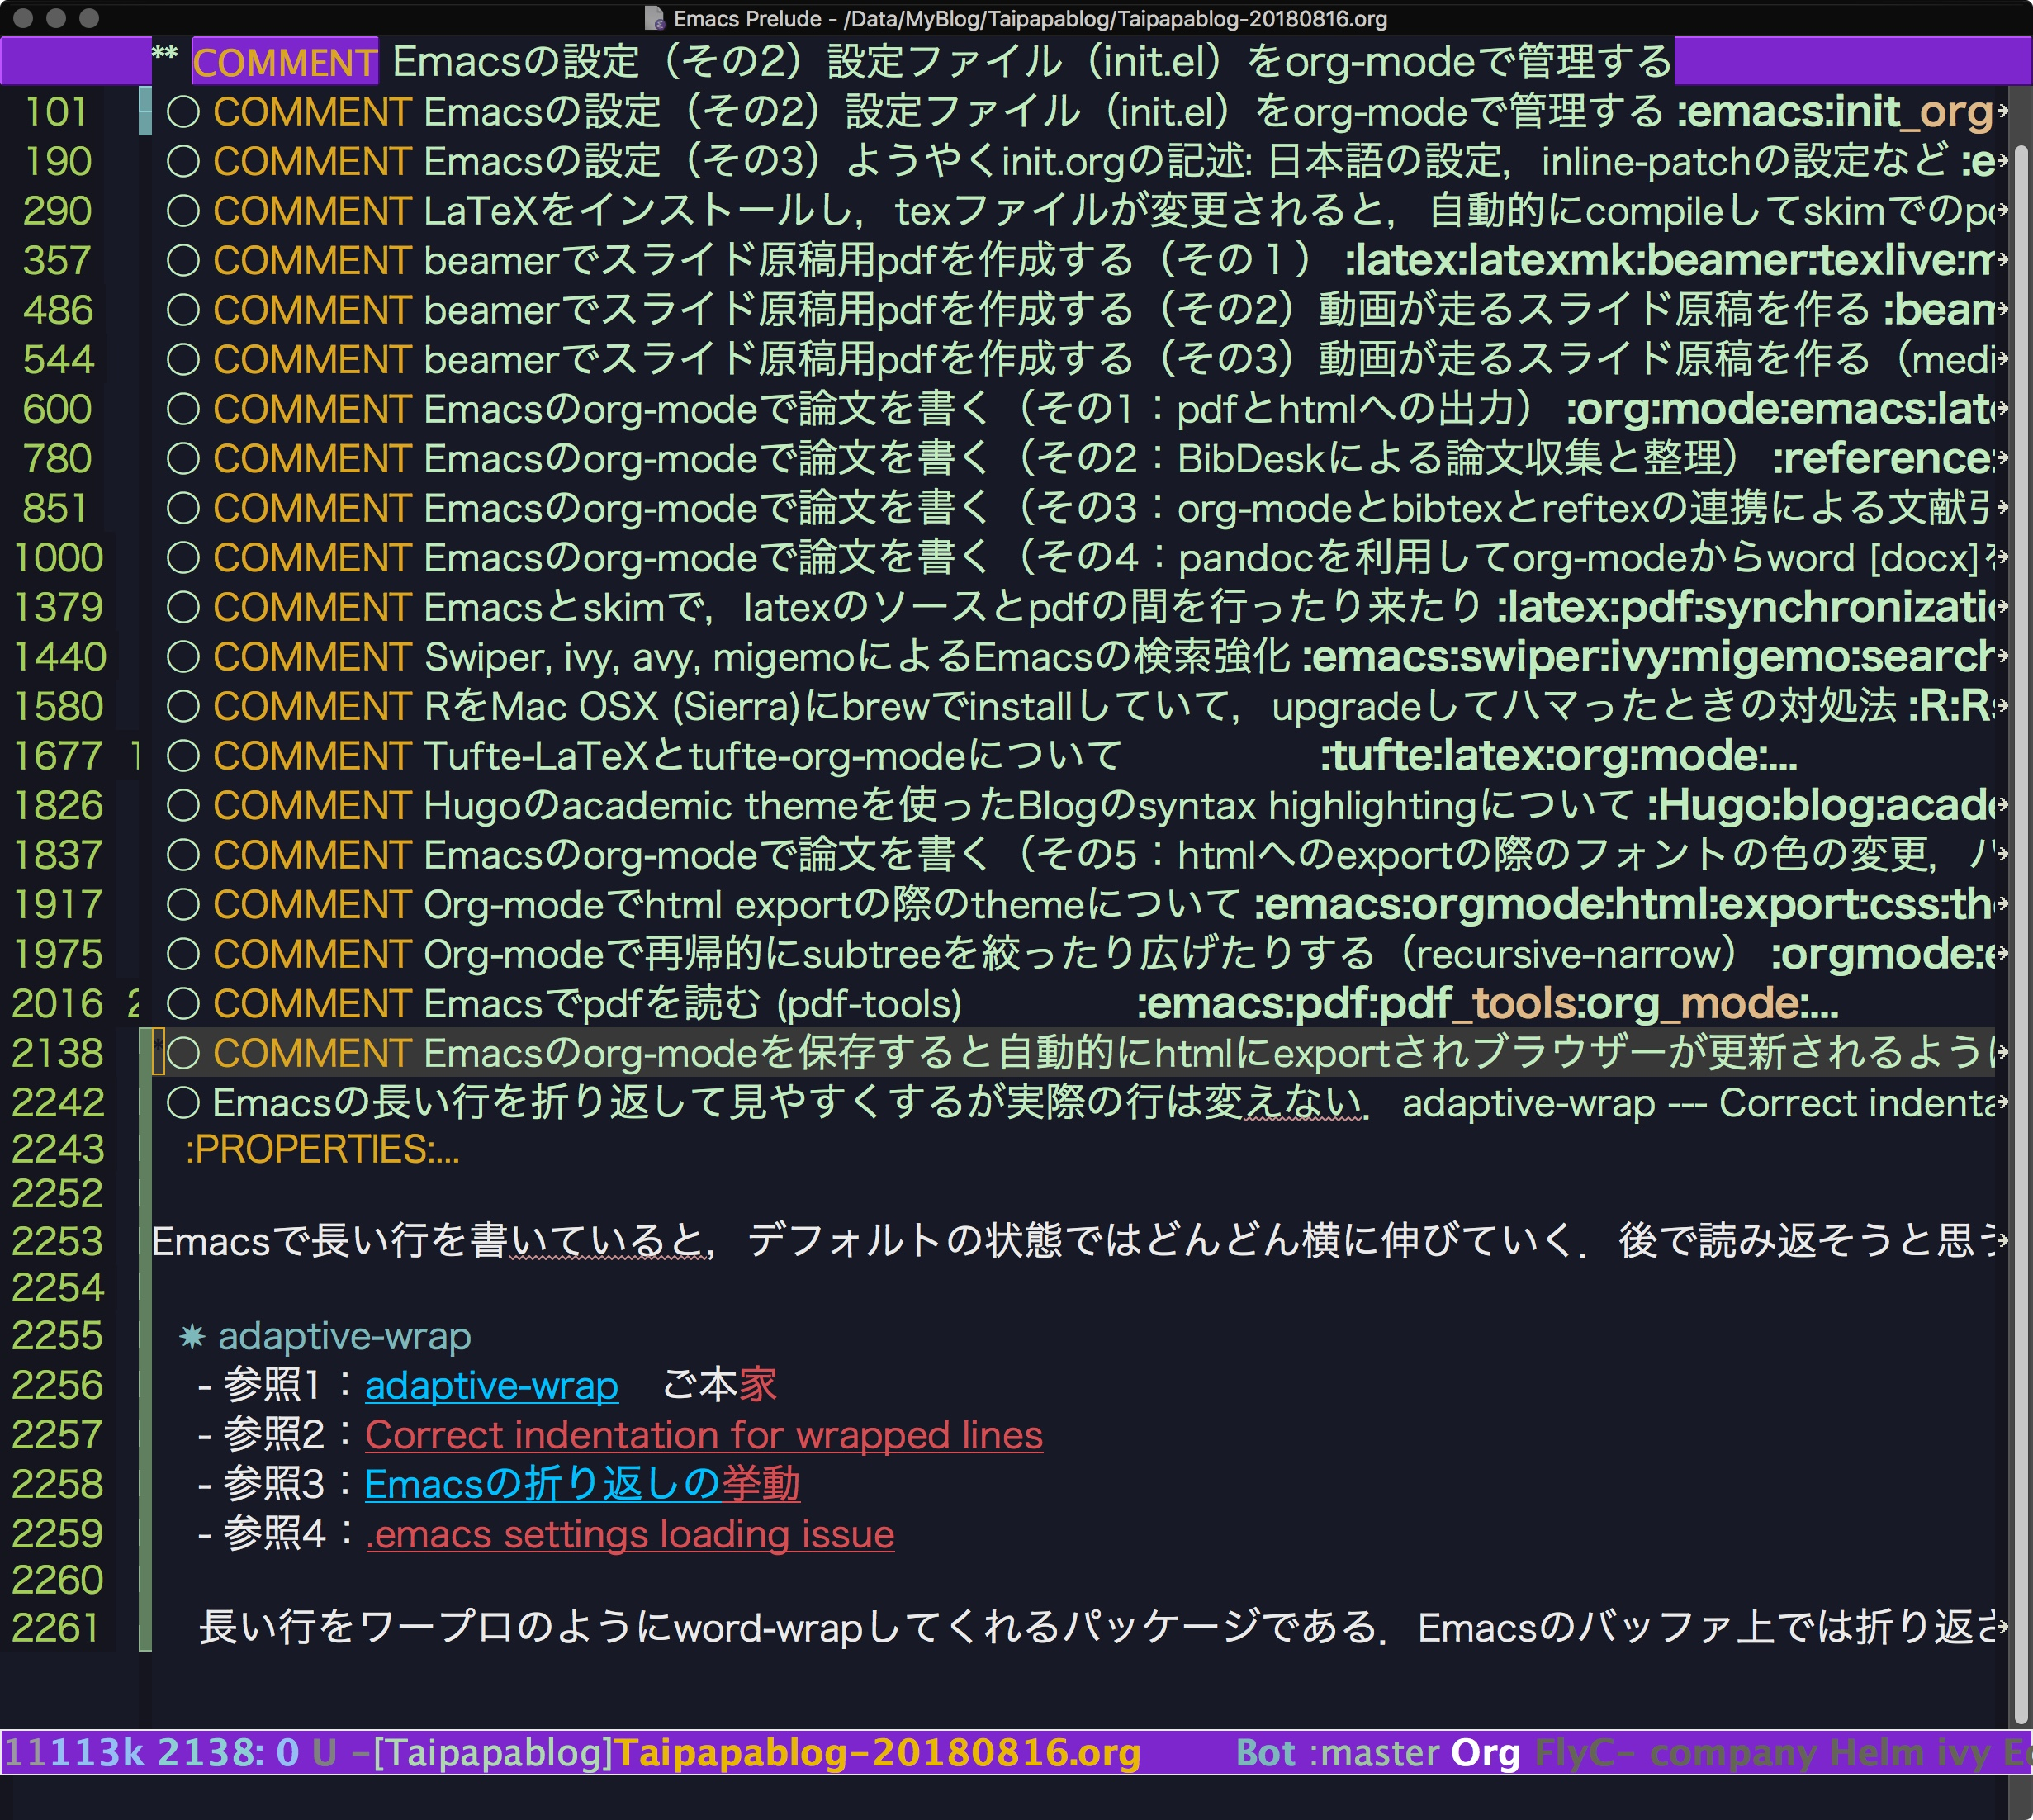
\includegraphics[width=.9\linewidth]{./static/img/Before_adaptive.jpg}

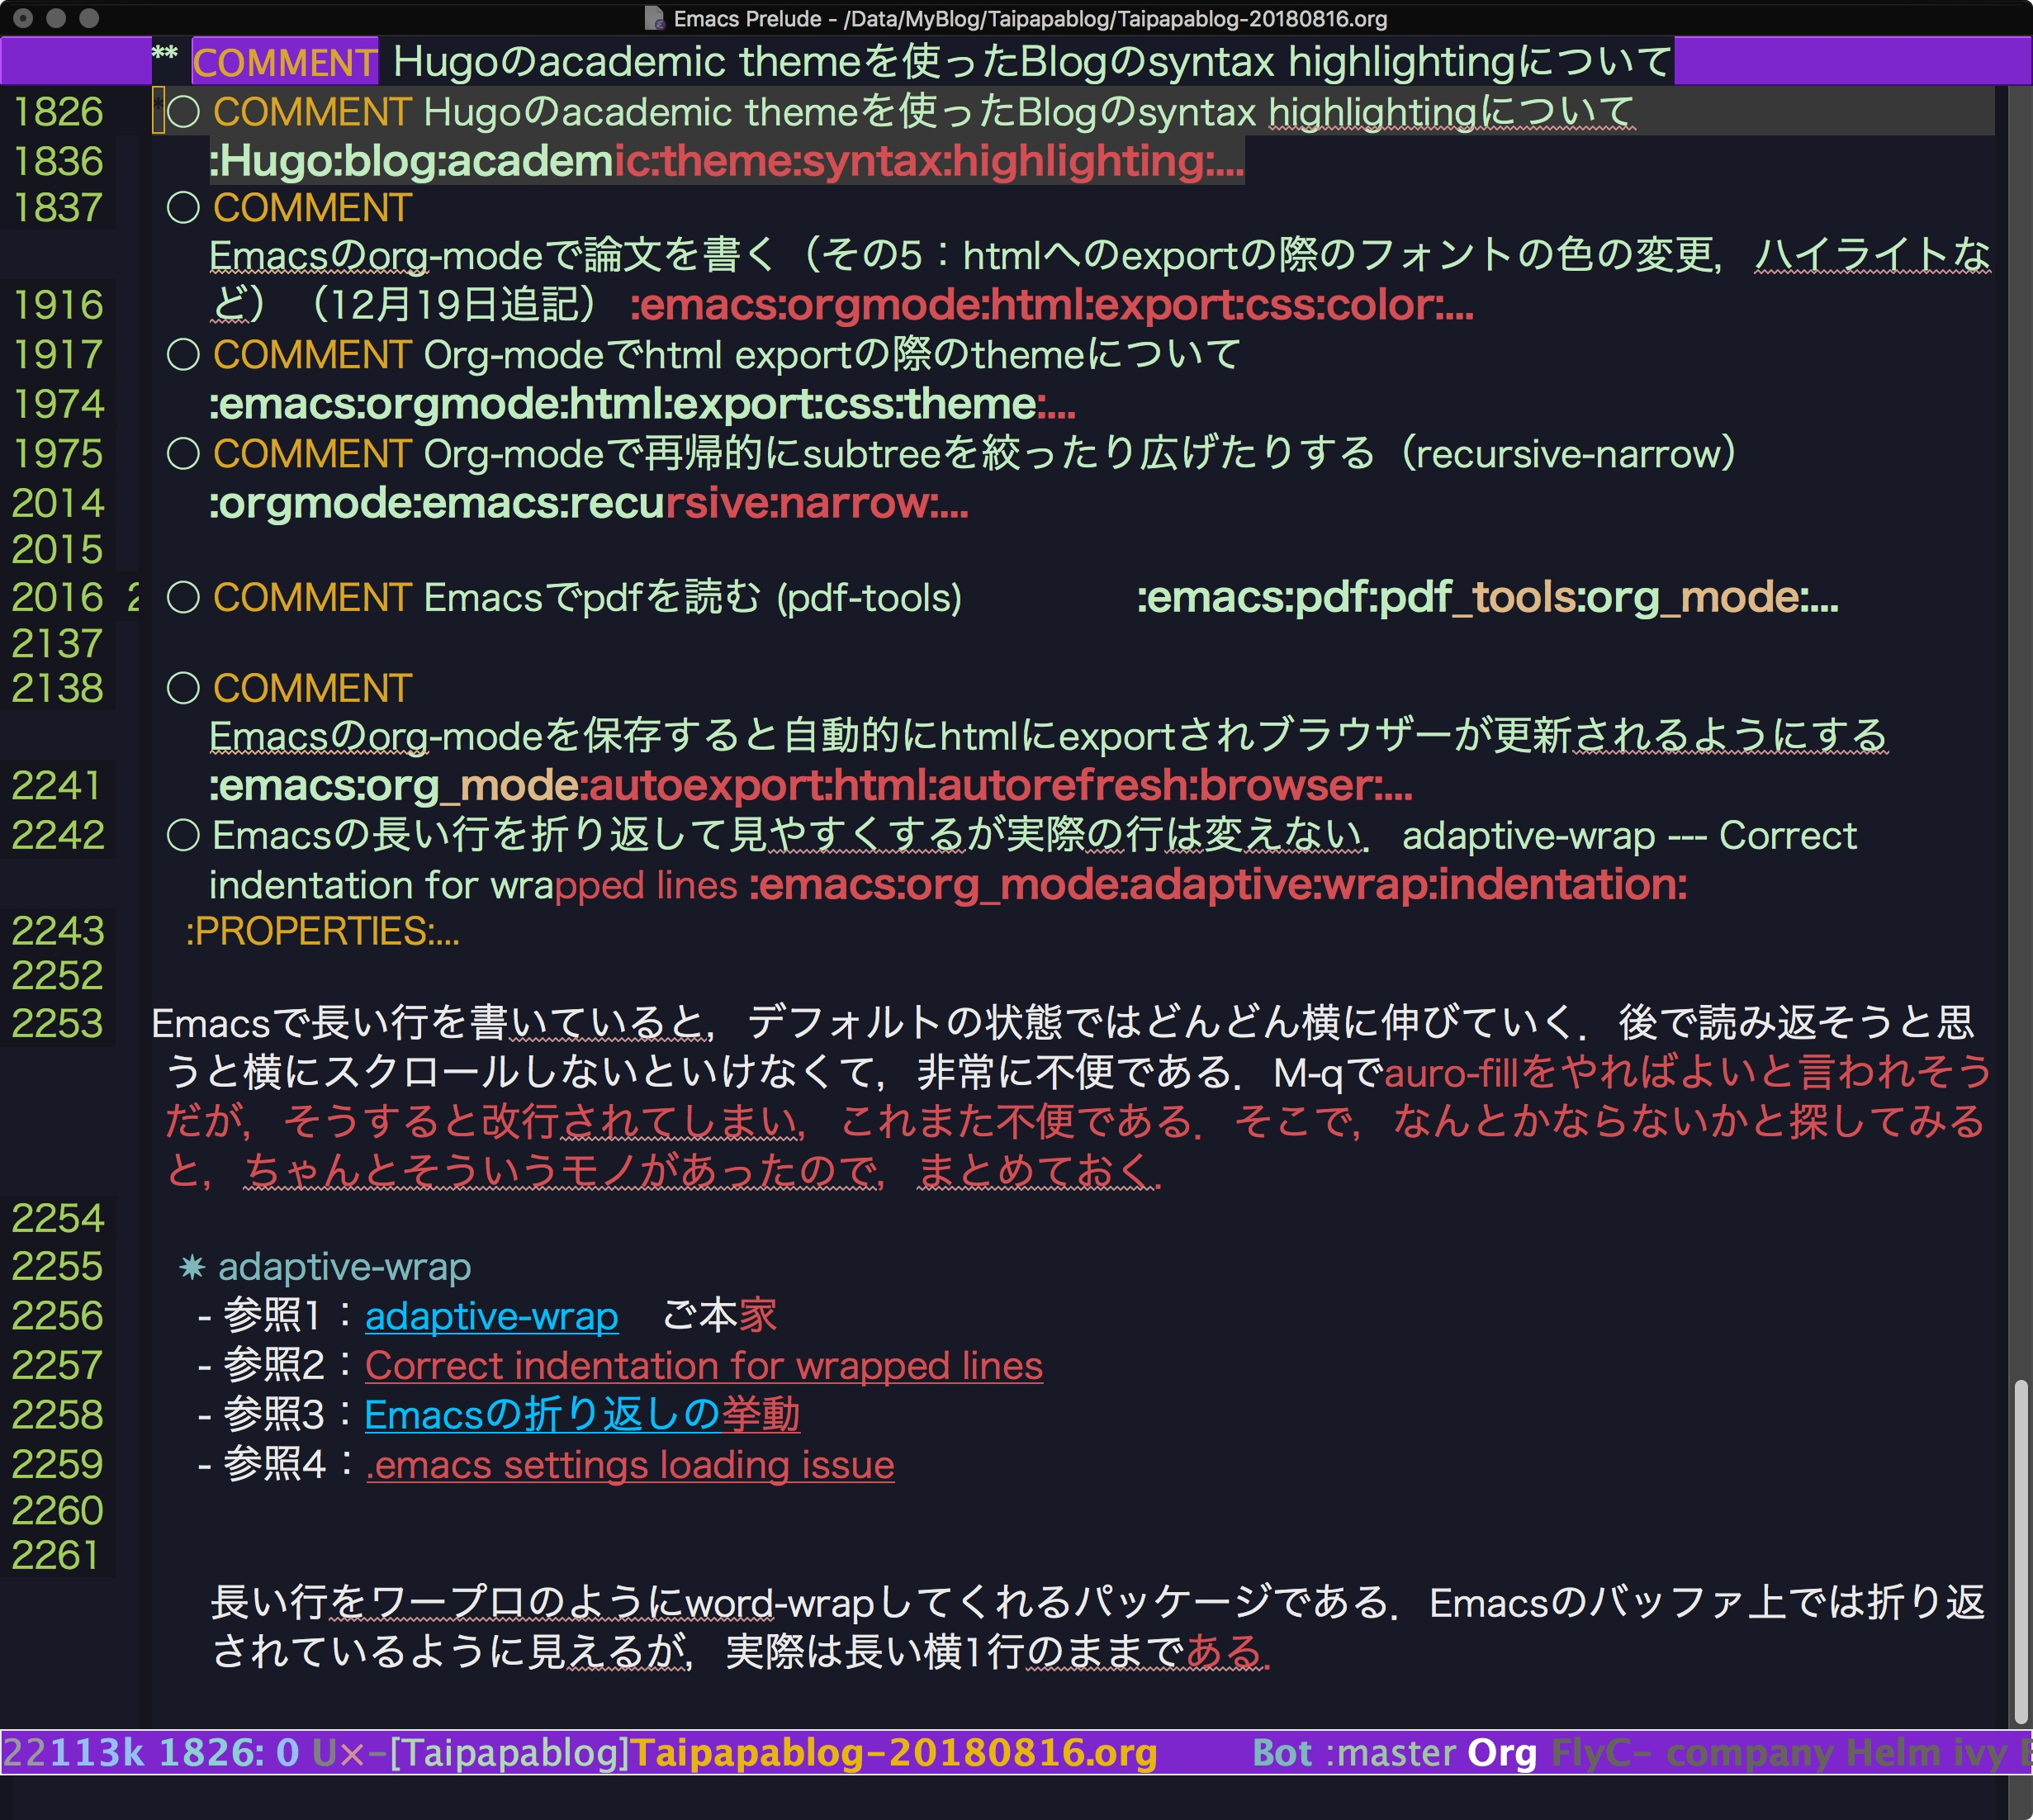
\includegraphics[width=.9\linewidth]{./static/img/After_adaptive.jpg}



([[../org-mode\(_{\text{paper}}\)\(_{\text{2}}\)][Emacsのorg-modeで論文を書く(その2:BibDeskによる論文収集と整理)]
\end{enumerate}
\end{document}
